
\subsection{Amplificadores con operacionales}

\label{section:modelo_operacional}

En esta sección analizamos distintas configuraciones con amplificadores operacionales, pero teniendo en cuenta ciertos aspectos de los amplificadores operacionales reales, en particular usamos un modelo lineal, y lo analizamos a bajas/medias frecuencias, sin tener en cuenta en principio el ancho de banda, ni cosas como el \textit{slew rate}, que corresponden a efectos que no se pueden modelar linealmente. El modelo utilizado es el mostrado en la figura~\figref{fig:fig_operational_non_ideal}, como se puede ver, solo consideramos, una ganancia de tensión diferencial de valor finito, una resistencia de entrada también finita y una resistencia de salida mayor a $0$.

\begin{figure}[H] %htb
\begin{center}
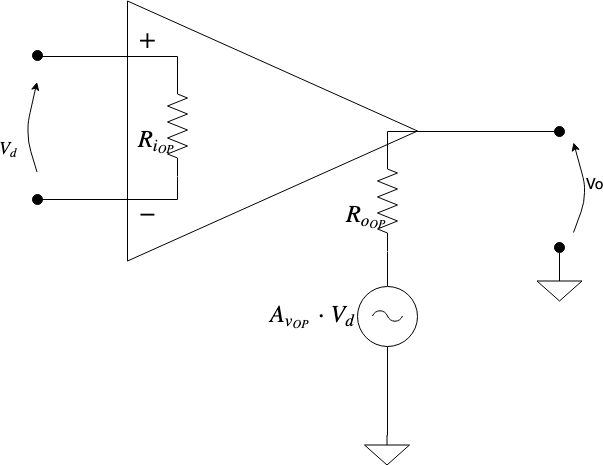
\includegraphics[width=1 \textwidth, angle=0]{./img/operacionales/OP_NONIDEAL_MODEL.png}
\caption{\label{fig:fig_operational_non_ideal}\footnotesize{Modelo lineal de un operacional no ideal.}}
\end{center}
\end{figure}

\vfill

\clearpage

\subsubsection{Amplificador no inversor}

Usando el modelo descripto en la sección~\sectref{section:modelo_operacional} analizamos el circuito mostrado en la figura~\figref{fig:fig_operational_ideal_non_inverter}. El circuito es un amplificador no inversor con amplificador operacional. El análisis que se hará por realimentación, pretende analizar como es la transferencia de mismo con nuestro modelo, y como influye la no idealidad del operacional en la transferencia, para finalmente ver a que se reduce la transferencia al llevar las expresiones al caso ideal.

\begin{figure}[H] %htb
\begin{center}
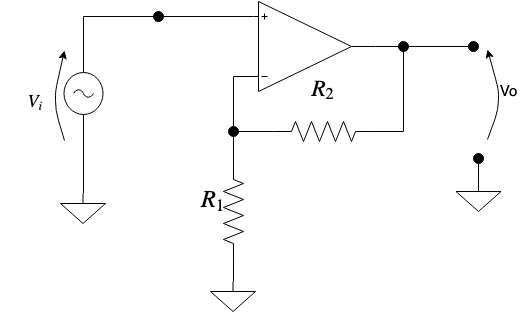
\includegraphics[width=0.5 \textwidth, angle=0]{./img/operacionales/OP_NINV.png}
\caption{\label{fig:fig_operational_ideal_non_inverter}\footnotesize{Amplificador no inversor.}}
\end{center}
\end{figure}

El amplificador amplifica de tensión, para ver esto, se observa que la red de realimentación formada por $R_{1}$ y $R_{2}$, muestrea la tensión a la salida y suma (resta) tensión a la entrada, con lo que se estabiliza la ganancia de tensión. Ya que se trata de realimentación \textbf{serie-paralelo} aplicamos parámetros \textbf{h} al realimentador.



\begin{figure}[H] %htb
\begin{center}
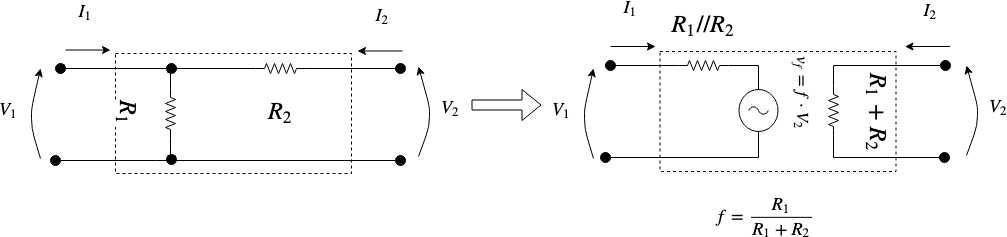
\includegraphics[width=0.9 \textwidth, angle=0]{./img/operacionales/OP_NINV_FEEDBACK.png}
\caption{\label{fig:fig_ninv_feedback}\footnotesize{Aplicando parámetros \textbf{h} al realimentador}}
\end{center}
\end{figure}



Remplazando en el circuito nuestro modelo y el realimentador por el modelo en parámetros \textbf{h}, y reorganizando para llevar el realimentador a su forma ideal, nos queda:


\begin{figure}[H] %htb
\begin{center}
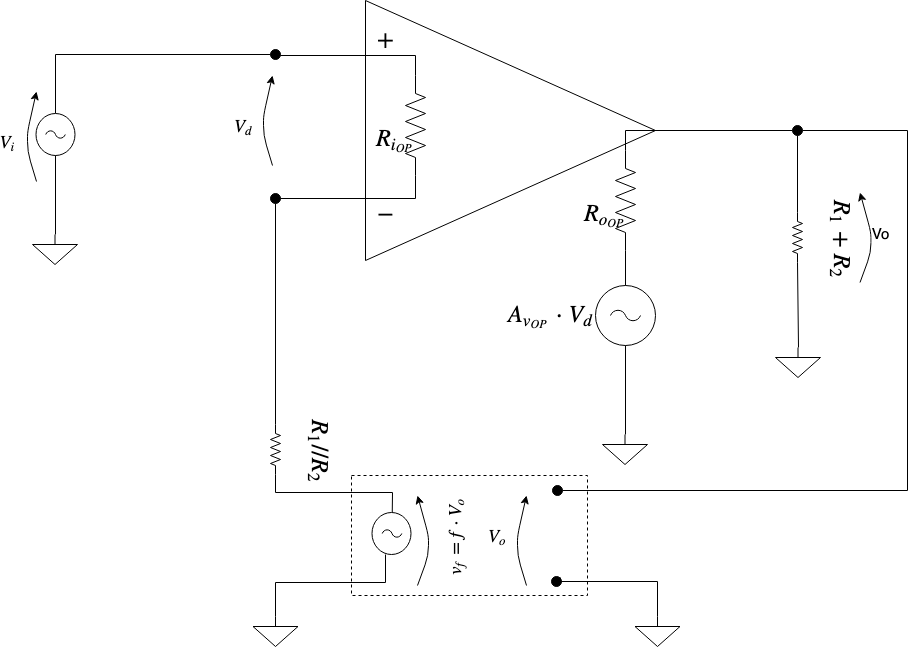
\includegraphics[width=0.9 \textwidth, angle=0]{./img/operacionales/OP_NONIDEAL_MODEL_NINV_FEEDBACK_PARAMETERS.png}
\caption{\label{fig:fig_nideal_ninv_feedback_pars}\footnotesize{Reemplazando en el circuito original junto a nuestro modelo}}
\end{center}
\end{figure}

De este circuito es fácil por inspección obtener la ganancia de tensión a lazo abierto, \quotemarks{a} y las resistencias de entrada y salida a lazo abierto, $R{i_{OL}}$ y $R{o_{OL}}$ respectivamente, se obtiene:


\begin{equation}
a =  \evalat{\frac{V_{o}}{V_{i}}}{f=0} = A_{v_{OP}} \cdot \frac{R_{i_{OP}}}{R_{i_{OP}} + R{1} \parallelresistors R{2} } \cdot \frac{ R_{1} + R_{2}}{R_{o_{OP}} + R_{1} + R_{2} }
\end{equation}

\begin{equation}
f =  \frac{R_{1}}{R_{1} + R_{2}}
\end{equation}

\begin{equation}
R_{i_{OL}} = R_{i_{OP}} + R{1} \parallelresistors R{2}
\end{equation}

\begin{equation}
R_{o_{OL}} = \left( R_{1} + R{2} \right) \parallelresistors R_{o_{OP}}
\end{equation}

Para la ganancia de tensión a lazo cerrado y las resistencias de entrada y salida a lazo cerrado, $R{i}$ y $R{o}$ respectivamente, entonces tenemos:


\begin{equation}
\boxed{ A = \frac{a}{1 + a \cdot f} = \frac{R_{1} + R{2}}{ \left( 1 + \frac{R{1} \parallelresistors R{2}}{R_{i_{OP}}} \right) \cdot \left( \frac{R_{o_{OP}} + R_{1} + R_{2}}{A_{v_{OP}}} + R_{1} \right) } }
\end{equation}


\begin{equation}
\boxed{ R{i} = R_{i_{OL}} \cdot \left( 1 + a \cdot f \right) = \left(  R_{i_{OP}} + R{1} \parallelresistors R{2} \right) \cdot \left[ 1 + \frac{ A_{v_{OP}} \cdot R_{1} \cdot R_{i_{OP}} }{  \left( R_{i_{OP}} + R{1} \parallelresistors R{2} \right) \cdot \left( R_{o_{OP}} + R_{1} + R_{2} \right) } \right] }
\end{equation}


\begin{equation}
\boxed{ R{o} = \frac{R_{o_{OL}}}{1 + a \cdot f} = \frac{\left( R_{1} + R{2} \right) \parallelresistors R_{o_{OP}}}{1 + \frac{ A_{v_{OP}} \cdot R_{1} \cdot R_{i_{OP}} }{  \left( R_{i_{OP}} + R{1} \parallelresistors R{2} \right) \cdot \left( R_{o_{OP}} + R_{1} + R_{2} \right) }} }
\end{equation}


Se obtiene para el caso ideal, cuando $A_{v_{OP}} \longrightarrow \infty$, $R_{i_{OP}} \longrightarrow \infty$ y $R_{o_{OP}} \longrightarrow 0$:

\begin{equation}
\lim_{\substack{A_{v_{OP}} \to \infty \\ R_{i_{OP}} \to \infty \\ R_{o_{OP}} \to 0}} A = 1 + \frac{R_{2}}{R_{1}} 
\end{equation}


\begin{equation}
\lim_{\substack{A_{v_{OP}} \to \infty \\ R_{i_{OP}} \to \infty \\ R_{o_{OP}} \to 0}} R{i} = \infty
\end{equation}


\begin{equation}
\lim_{\substack{A_{v_{OP}} \to \infty \\ R_{i_{OP}} \to \infty \\ R_{o_{OP}} \to 0}} R{o} = 0
\end{equation}

Queda ver en cada caso cuando estas aproximaciones son válidas, por ejemplo para el caso del \textit{TL082}, (valores tomados de su hoja de datos~\sectref{datasheet_TL082}), se tiene:

\begin{equation}
\min A_{v_{OP}} \approx 25000
\end{equation}


\begin{equation}
\min R_{i_{OP}} \approx 1 \si[per-mode=symbol]{\tera\ohm}
\end{equation}


\begin{equation}
\max R_{o_{OP}} \approx 100 \si[per-mode=symbol]{\ohm}
\end{equation}

Se puede ver de las expresiones halladas antes, que la ganancia a lazo abierto, \quotemarks{$a$}, será aproximadamente la ganancia de tensión del amplificador operacional, así que en general para valores de resistencias de realimentación en el orden algunos $\si[per-mode=symbol]{\kilo\ohm}$ y valores de realimentación no muy grandes, estas aproximaciones serán muy buenas.



\subsubsection{Amplificador inversor}


\subsubsection{Amplificador diferencial}